
%% !TEX root = manual.tex

\section{Spyplot Diagrams}
\label{sec:tutorials:spyplot}

Spyplots visualize communication matrices, showing either the number of messages or number of bytes sent between two network endpoints.
They are essentially contour diagrams, where instead of a continuous function $F(x,y)$ we are plotting the communication matrix $M(i,j)$.
An example spyplot is shown for a simple application that only executes an MPI\_Allreduce (Figure \ref{fig:spyplot}).
Larger amounts of data (red) are sent to nearest neighbors while decreasing amounts (blue) are sent to MPI ranks further away.

\begin{figure}[h]
\centering
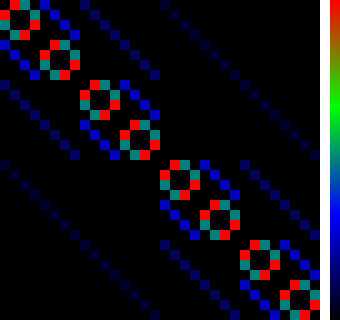
\includegraphics[width=0.4\textwidth]{figures/spyplot/mpi_spyplot.png}
\caption{Spyplot of Bytes Transferred Between MPI Ranks for MPI\_Allreduce}
\label{fig:spyplot}
\end{figure}

Various spyplots can be activated.
The most commonly used are the MPI spyplots, for which you activate the spyplot as part of the MPI subcomponent.

\begin{ViFile}
node {
  app1 {
    mpi {
      spy_bytes {
        type = spyplot
        output = csv
        group = app1
      }
    }
  }
}
\end{ViFile}
After running, there will be a CSV containing the data sent by each component to another component.
The same statistic can be activated in both the \inlinecode{node.app1.mpi} namespaces and the \inlinecode{node.nic} namespaces.
The type of the statistic must be spyplot, but the output can be other formats (but just use csv).

